% Options for packages loaded elsewhere
\PassOptionsToPackage{unicode}{hyperref}
\PassOptionsToPackage{hyphens}{url}
%
\documentclass[
  12pt,
]{article}
\usepackage{amsmath,amssymb}
\usepackage{lmodern}
\usepackage{ifxetex,ifluatex}
\ifnum 0\ifxetex 1\fi\ifluatex 1\fi=0 % if pdftex
  \usepackage[T1]{fontenc}
  \usepackage[utf8]{inputenc}
  \usepackage{textcomp} % provide euro and other symbols
\else % if luatex or xetex
  \usepackage{unicode-math}
  \defaultfontfeatures{Scale=MatchLowercase}
  \defaultfontfeatures[\rmfamily]{Ligatures=TeX,Scale=1}
\fi
% Use upquote if available, for straight quotes in verbatim environments
\IfFileExists{upquote.sty}{\usepackage{upquote}}{}
\IfFileExists{microtype.sty}{% use microtype if available
  \usepackage[]{microtype}
  \UseMicrotypeSet[protrusion]{basicmath} % disable protrusion for tt fonts
}{}
\makeatletter
\@ifundefined{KOMAClassName}{% if non-KOMA class
  \IfFileExists{parskip.sty}{%
    \usepackage{parskip}
  }{% else
    \setlength{\parindent}{0pt}
    \setlength{\parskip}{6pt plus 2pt minus 1pt}}
}{% if KOMA class
  \KOMAoptions{parskip=half}}
\makeatother
\usepackage{xcolor}
\IfFileExists{xurl.sty}{\usepackage{xurl}}{} % add URL line breaks if available
\IfFileExists{bookmark.sty}{\usepackage{bookmark}}{\usepackage{hyperref}}
\hypersetup{
  pdftitle={Lab 2 - Bayesian Statistics - Distributional Theory},
  pdfauthor={Daniel Carpenter},
  hidelinks,
  pdfcreator={LaTeX via pandoc}}
\urlstyle{same} % disable monospaced font for URLs
\usepackage[margin=1in]{geometry}
\usepackage{color}
\usepackage{fancyvrb}
\newcommand{\VerbBar}{|}
\newcommand{\VERB}{\Verb[commandchars=\\\{\}]}
\DefineVerbatimEnvironment{Highlighting}{Verbatim}{commandchars=\\\{\}}
% Add ',fontsize=\small' for more characters per line
\usepackage{framed}
\definecolor{shadecolor}{RGB}{248,248,248}
\newenvironment{Shaded}{\begin{snugshade}}{\end{snugshade}}
\newcommand{\AlertTok}[1]{\textcolor[rgb]{0.94,0.16,0.16}{#1}}
\newcommand{\AnnotationTok}[1]{\textcolor[rgb]{0.56,0.35,0.01}{\textbf{\textit{#1}}}}
\newcommand{\AttributeTok}[1]{\textcolor[rgb]{0.77,0.63,0.00}{#1}}
\newcommand{\BaseNTok}[1]{\textcolor[rgb]{0.00,0.00,0.81}{#1}}
\newcommand{\BuiltInTok}[1]{#1}
\newcommand{\CharTok}[1]{\textcolor[rgb]{0.31,0.60,0.02}{#1}}
\newcommand{\CommentTok}[1]{\textcolor[rgb]{0.56,0.35,0.01}{\textit{#1}}}
\newcommand{\CommentVarTok}[1]{\textcolor[rgb]{0.56,0.35,0.01}{\textbf{\textit{#1}}}}
\newcommand{\ConstantTok}[1]{\textcolor[rgb]{0.00,0.00,0.00}{#1}}
\newcommand{\ControlFlowTok}[1]{\textcolor[rgb]{0.13,0.29,0.53}{\textbf{#1}}}
\newcommand{\DataTypeTok}[1]{\textcolor[rgb]{0.13,0.29,0.53}{#1}}
\newcommand{\DecValTok}[1]{\textcolor[rgb]{0.00,0.00,0.81}{#1}}
\newcommand{\DocumentationTok}[1]{\textcolor[rgb]{0.56,0.35,0.01}{\textbf{\textit{#1}}}}
\newcommand{\ErrorTok}[1]{\textcolor[rgb]{0.64,0.00,0.00}{\textbf{#1}}}
\newcommand{\ExtensionTok}[1]{#1}
\newcommand{\FloatTok}[1]{\textcolor[rgb]{0.00,0.00,0.81}{#1}}
\newcommand{\FunctionTok}[1]{\textcolor[rgb]{0.00,0.00,0.00}{#1}}
\newcommand{\ImportTok}[1]{#1}
\newcommand{\InformationTok}[1]{\textcolor[rgb]{0.56,0.35,0.01}{\textbf{\textit{#1}}}}
\newcommand{\KeywordTok}[1]{\textcolor[rgb]{0.13,0.29,0.53}{\textbf{#1}}}
\newcommand{\NormalTok}[1]{#1}
\newcommand{\OperatorTok}[1]{\textcolor[rgb]{0.81,0.36,0.00}{\textbf{#1}}}
\newcommand{\OtherTok}[1]{\textcolor[rgb]{0.56,0.35,0.01}{#1}}
\newcommand{\PreprocessorTok}[1]{\textcolor[rgb]{0.56,0.35,0.01}{\textit{#1}}}
\newcommand{\RegionMarkerTok}[1]{#1}
\newcommand{\SpecialCharTok}[1]{\textcolor[rgb]{0.00,0.00,0.00}{#1}}
\newcommand{\SpecialStringTok}[1]{\textcolor[rgb]{0.31,0.60,0.02}{#1}}
\newcommand{\StringTok}[1]{\textcolor[rgb]{0.31,0.60,0.02}{#1}}
\newcommand{\VariableTok}[1]{\textcolor[rgb]{0.00,0.00,0.00}{#1}}
\newcommand{\VerbatimStringTok}[1]{\textcolor[rgb]{0.31,0.60,0.02}{#1}}
\newcommand{\WarningTok}[1]{\textcolor[rgb]{0.56,0.35,0.01}{\textbf{\textit{#1}}}}
\usepackage{graphicx}
\makeatletter
\def\maxwidth{\ifdim\Gin@nat@width>\linewidth\linewidth\else\Gin@nat@width\fi}
\def\maxheight{\ifdim\Gin@nat@height>\textheight\textheight\else\Gin@nat@height\fi}
\makeatother
% Scale images if necessary, so that they will not overflow the page
% margins by default, and it is still possible to overwrite the defaults
% using explicit options in \includegraphics[width, height, ...]{}
\setkeys{Gin}{width=\maxwidth,height=\maxheight,keepaspectratio}
% Set default figure placement to htbp
\makeatletter
\def\fps@figure{htbp}
\makeatother
\setlength{\emergencystretch}{3em} % prevent overfull lines
\providecommand{\tightlist}{%
  \setlength{\itemsep}{0pt}\setlength{\parskip}{0pt}}
\setcounter{secnumdepth}{5}
\ifluatex
  \usepackage{selnolig}  % disable illegal ligatures
\fi

\title{Lab 2 - Bayesian Statistics - Distributional Theory}
\author{Daniel Carpenter}
\date{January 2022}

\begin{document}
\maketitle

{
\setcounter{tocdepth}{2}
\tableofcontents
}
\begin{center}\rule{0.5\linewidth}{0.5pt}\end{center}

\hypertarget{discrete-binomial-distribution}{%
\section{Discrete Binomial
Distribution}\label{discrete-binomial-distribution}}

\begin{quote}
\emph{Note} that the discrete binomial distribution is very useful for
modeling processes in which the binary outcome can be
\textbf{\emph{either}} a success (\texttt{1}, \texttt{TRUE}) or a
failure (\texttt{0}, \texttt{FALSE})
\end{quote}

\hypertarget{latex-formula-for-discrete-binomial-distribution}{%
\subsubsection{\texorpdfstring{\texttt{LaTex} Formula for Discrete
Binomial
Distribution}{LaTex Formula for Discrete Binomial Distribution}}\label{latex-formula-for-discrete-binomial-distribution}}

\[
p(X = x|n, p) = 
  \begin{pmatrix}
  N \\
  k 
  \end{pmatrix}
p^k(1-p)^{N - k}
\]

\hypertarget{function-dmybin-to-calculate-discrete-binomial-distribition}{%
\subsubsection{\texorpdfstring{Function (\texttt{dmybin}) to Calculate
Discrete Binomial
Distribition}{Function (dmybin) to Calculate Discrete Binomial Distribition}}\label{function-dmybin-to-calculate-discrete-binomial-distribition}}

\begin{Shaded}
\begin{Highlighting}[]
\NormalTok{dmybin }\OtherTok{\textless{}{-}} \ControlFlowTok{function}\NormalTok{(X, n, p) \{}
  
  \CommentTok{\# Change X to k to be consistent with textbook}
\NormalTok{  k }\OtherTok{=}\NormalTok{ X}
  
  \CommentTok{\# Calculate the binomial coefficient (N k)}
\NormalTok{  binomialCoefficient }\OtherTok{\textless{}{-}} \FunctionTok{choose}\NormalTok{(n, X)}
  
  \CommentTok{\# Return the discrete binomial calculation}
  \FunctionTok{return}\NormalTok{(binomialCoefficient }\SpecialCharTok{*}\NormalTok{ p}\SpecialCharTok{\^{}}\NormalTok{k }\SpecialCharTok{*}\NormalTok{ (}\DecValTok{1} \SpecialCharTok{{-}}\NormalTok{ p)}\SpecialCharTok{\^{}}\NormalTok{(n }\SpecialCharTok{{-}}\NormalTok{ k))}
\NormalTok{\}}
\end{Highlighting}
\end{Shaded}

\hypertarget{call-and-return-results-of-the-dmybin-function}{%
\subsubsection{\texorpdfstring{Call and Return Results of the
\texttt{dmybin}
Function}{Call and Return Results of the dmybin Function}}\label{call-and-return-results-of-the-dmybin-function}}

\begin{Shaded}
\begin{Highlighting}[]
\NormalTok{y.dmybin }\OtherTok{=} \FunctionTok{dmybin}\NormalTok{(}\AttributeTok{X=}\DecValTok{0}\SpecialCharTok{:}\DecValTok{4}\NormalTok{, }\AttributeTok{n=}\DecValTok{10}\NormalTok{, }\AttributeTok{p=}\FloatTok{0.5}\NormalTok{)}
\NormalTok{y.dmybin}
\end{Highlighting}
\end{Shaded}

\begin{verbatim}
## [1] 0.0009765625 0.0097656250 0.0439453125 0.1171875000 0.2050781250
\end{verbatim}

\hypertarget{call-and-return-results-of-base-r-binomial-distribution-function-dbinom}{%
\subsubsection{\texorpdfstring{Call and Return Results of \texttt{base}
R Binomial Distribution Function
\texttt{dbinom}}{Call and Return Results of base R Binomial Distribution Function dbinom}}\label{call-and-return-results-of-base-r-binomial-distribution-function-dbinom}}

\begin{Shaded}
\begin{Highlighting}[]
\NormalTok{y.dbinom }\OtherTok{=} \FunctionTok{dbinom}\NormalTok{(}\AttributeTok{x=}\DecValTok{0}\SpecialCharTok{:}\DecValTok{4}\NormalTok{, }\AttributeTok{size=}\DecValTok{10}\NormalTok{, }\AttributeTok{prob=}\FloatTok{0.5}\NormalTok{)}
\NormalTok{y.dbinom}
\end{Highlighting}
\end{Shaded}

\begin{verbatim}
## [1] 0.0009765625 0.0097656250 0.0439453125 0.1171875000 0.2050781250
\end{verbatim}

\begin{center}\rule{0.5\linewidth}{0.5pt}\end{center}

\hypertarget{create-a-cumulative-probability-function-called-pmybin}{%
\subsubsection{\texorpdfstring{Create a Cumulative Probability Function
Called
\texttt{pmybin}}{Create a Cumulative Probability Function Called pmybin}}\label{create-a-cumulative-probability-function-called-pmybin}}

\begin{Shaded}
\begin{Highlighting}[]
\NormalTok{pmybin }\OtherTok{\textless{}{-}} \ControlFlowTok{function}\NormalTok{(dmybin, x, n, p) \{}
  
  \CommentTok{\# Return the Cumulative Probability}
  \FunctionTok{return}\NormalTok{(}\FunctionTok{sum}\NormalTok{(}\FunctionTok{dmybin}\NormalTok{(}\DecValTok{0}\SpecialCharTok{:}\NormalTok{x, n, p)))}
\NormalTok{\}}
\end{Highlighting}
\end{Shaded}

\hypertarget{call-and-return-results-of-the-pmybin}{%
\subsubsection{\texorpdfstring{Call and Return Results of the
\texttt{pmybin}}{Call and Return Results of the pmybin}}\label{call-and-return-results-of-the-pmybin}}

\begin{Shaded}
\begin{Highlighting}[]
\NormalTok{cumulativeProbability.pmybin }\OtherTok{\textless{}{-}} \FunctionTok{pmybin}\NormalTok{(dmybin, }\AttributeTok{x=}\DecValTok{5}\NormalTok{, }\AttributeTok{n=}\DecValTok{10}\NormalTok{, }\AttributeTok{p=}\FloatTok{0.5}\NormalTok{)}
\NormalTok{cumulativeProbability.pmybin}
\end{Highlighting}
\end{Shaded}

\begin{verbatim}
## [1] 0.6230469
\end{verbatim}

\hypertarget{call-and-return-results-of-base-r-binomial-function-distribution-function-pbinom}{%
\subsubsection{\texorpdfstring{Call and Return Results of \texttt{base}
R Binomial Function Distribution Function
\texttt{pbinom}}{Call and Return Results of base R Binomial Function Distribution Function pbinom}}\label{call-and-return-results-of-base-r-binomial-function-distribution-function-pbinom}}

\begin{Shaded}
\begin{Highlighting}[]
\NormalTok{cumulativeProbability.pbinom }\OtherTok{\textless{}{-}} \FunctionTok{pbinom}\NormalTok{(}\AttributeTok{q =} \DecValTok{5}\NormalTok{, }\AttributeTok{size=}\DecValTok{10}\NormalTok{, }\AttributeTok{prob=}\FloatTok{0.5}\NormalTok{)}
\NormalTok{cumulativeProbability.pbinom}
\end{Highlighting}
\end{Shaded}

\begin{verbatim}
## [1] 0.6230469
\end{verbatim}

\hypertarget{create-a-binomial-distribution-plot}{%
\subsubsection{Create a Binomial Distribution
Plot}\label{create-a-binomial-distribution-plot}}

\begin{Shaded}
\begin{Highlighting}[]
\NormalTok{x }\OtherTok{=} \DecValTok{0}\SpecialCharTok{:}\DecValTok{10}

\FunctionTok{plot}\NormalTok{(x, }
     \AttributeTok{y =} \FunctionTok{dbinom}\NormalTok{(x, }\AttributeTok{size =} \DecValTok{10}\NormalTok{, }\AttributeTok{prob =} \FloatTok{0.5}\NormalTok{),}
     \AttributeTok{type =} \StringTok{\textquotesingle{}h\textquotesingle{}}\NormalTok{, }\CommentTok{\# h := histogram like}
     \AttributeTok{main =} \StringTok{\textquotesingle{}Daniel Carpenter {-} Binomial Distributon\textquotesingle{}}\NormalTok{,}
     \AttributeTok{xlab =} \StringTok{\textquotesingle{}x\textquotesingle{}}\NormalTok{)}
\end{Highlighting}
\end{Shaded}

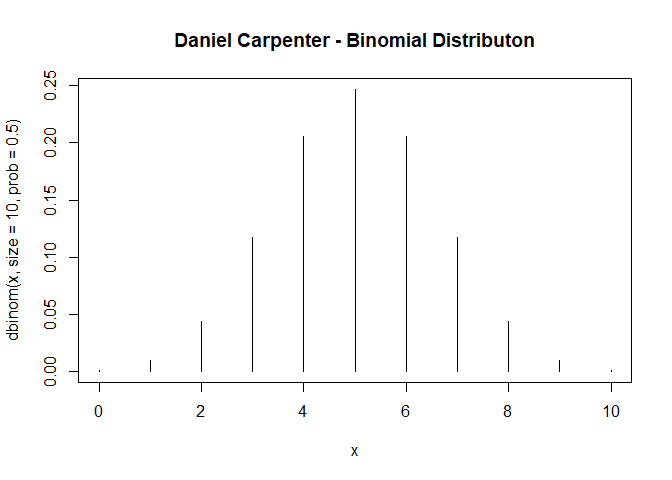
\includegraphics{lab2_files/figure-latex/bdist_plot-1.pdf}

\begin{center}\rule{0.5\linewidth}{0.5pt}\end{center}

\hypertarget{poisson-and-four-basic-distributional-functions-dpois-ppois-rpois-and-qpois}{%
\section{\texorpdfstring{Poisson and Four Basic Distributional
Functions: \texttt{dpois}, \texttt{ppois}, \texttt{rpois}, and
\texttt{qpois}}{Poisson and Four Basic Distributional Functions: dpois, ppois, rpois, and qpois}}\label{poisson-and-four-basic-distributional-functions-dpois-ppois-rpois-and-qpois}}

\hypertarget{a-poisson-calculations}{%
\subsection{\texorpdfstring{\texttt{a} Poisson
Calculations}{a Poisson Calculations}}\label{a-poisson-calculations}}

\hypertarget{find-ux1d443ux1d44b-4ux1d706-3}{%
\subsubsection{Find 𝑃(𝑋 = 4\textbar 𝜆 =
3)}\label{find-ux1d443ux1d44b-4ux1d706-3}}

\begin{itemize}
\tightlist
\item
  What is the probability that there are exactly 4 successes when 3 is
  the average?
\end{itemize}

\begin{Shaded}
\begin{Highlighting}[]
\FunctionTok{dpois}\NormalTok{(}\AttributeTok{x =} \DecValTok{4}\NormalTok{, }\AttributeTok{lambda =} \DecValTok{3}\NormalTok{)}
\end{Highlighting}
\end{Shaded}

\begin{verbatim}
## [1] 0.1680314
\end{verbatim}

\hypertarget{find-ux1d443ux1d44b-4ux1d706-3-1}{%
\subsubsection{Find 𝑃(𝑋 ≤ 4\textbar 𝜆 =
3)}\label{find-ux1d443ux1d44b-4ux1d706-3-1}}

\begin{itemize}
\tightlist
\item
  What is the probability that there are 4 or less successes when 3 is
  the average?
\end{itemize}

\begin{Shaded}
\begin{Highlighting}[]
\FunctionTok{ppois}\NormalTok{(}\AttributeTok{q =} \DecValTok{4}\NormalTok{, }\AttributeTok{lambda =} \DecValTok{3}\NormalTok{)}
\end{Highlighting}
\end{Shaded}

\begin{verbatim}
## [1] 0.8152632
\end{verbatim}

\hypertarget{find-ux1d443ux1d44b-4ux1d706-3-2}{%
\subsubsection{Find 𝑃(𝑋 \textgreater{} 4\textbar 𝜆 =
3)}\label{find-ux1d443ux1d44b-4ux1d706-3-2}}

\begin{itemize}
\tightlist
\item
  What is the probability that there are more than 4 successes when 3 is
  the average?
\end{itemize}

\begin{Shaded}
\begin{Highlighting}[]
\FunctionTok{ppois}\NormalTok{(}\AttributeTok{q =} \DecValTok{4}\NormalTok{, }\AttributeTok{lambda =} \DecValTok{3}\NormalTok{, }\AttributeTok{lower.tail =} \ConstantTok{FALSE}\NormalTok{)}
\end{Highlighting}
\end{Shaded}

\begin{verbatim}
## [1] 0.1847368
\end{verbatim}

\hypertarget{find-x-so-that-ux1d443ux1d44b-ux1d465ux1d706-3-0.9997077}{%
\subsubsection{Find x so that 𝑃(𝑋 ≤ 𝑥\textbar 𝜆 = 3)=
0.9997077}\label{find-x-so-that-ux1d443ux1d44b-ux1d465ux1d706-3-0.9997077}}

\begin{itemize}
\tightlist
\item
  How many successes when 3 on average and cumulative probability of
  0.9997077?
\end{itemize}

\begin{Shaded}
\begin{Highlighting}[]
\FunctionTok{qpois}\NormalTok{(}\AttributeTok{p =} \FloatTok{0.9997077}\NormalTok{, }\AttributeTok{lambda =} \DecValTok{3}\NormalTok{)}
\end{Highlighting}
\end{Shaded}

\begin{verbatim}
## [1] 11
\end{verbatim}

\hypertarget{create-a-sample-of-size-100-from-a-poisson-distribution-that-has-parameter-ux1d706-3.-store-in-an-object.}{%
\subsubsection{Create a sample of size 100 from a Poisson distribution
that has parameter 𝜆 = 3. Store in an
object.}\label{create-a-sample-of-size-100-from-a-poisson-distribution-that-has-parameter-ux1d706-3.-store-in-an-object.}}

\begin{Shaded}
\begin{Highlighting}[]
\NormalTok{poissonSample3 }\OtherTok{\textless{}{-}} \FunctionTok{rpois}\NormalTok{(}\AttributeTok{n =} \DecValTok{100}\NormalTok{, }\AttributeTok{lambda =} \DecValTok{3}\NormalTok{)}
\end{Highlighting}
\end{Shaded}

\hypertarget{make-a-second-sample-of-size-100-from-a-poisson-that-has-parameter-ux1d706-6-store-in-an-object}{%
\subsubsection{Make a second sample of size 100 from a Poisson that has
parameter 𝜆 = 6, store in an
object}\label{make-a-second-sample-of-size-100-from-a-poisson-that-has-parameter-ux1d706-6-store-in-an-object}}

\begin{Shaded}
\begin{Highlighting}[]
\NormalTok{poissonSample6 }\OtherTok{\textless{}{-}} \FunctionTok{rpois}\NormalTok{(}\AttributeTok{n =} \DecValTok{100}\NormalTok{, }\AttributeTok{lambda =} \DecValTok{6}\NormalTok{)}
\end{Highlighting}
\end{Shaded}

\hypertarget{bc-data-frame-and-base-ggplot-for-boxplots-and-violins}{%
\subsection{\texorpdfstring{\texttt{b/c} Data Frame and Base
\texttt{ggplot} for Boxplots and
Violins}{b/c Data Frame and Base ggplot for Boxplots and Violins}}\label{bc-data-frame-and-base-ggplot-for-boxplots-and-violins}}

\begin{Shaded}
\begin{Highlighting}[]
\ControlFlowTok{if}\NormalTok{(}\SpecialCharTok{!}\FunctionTok{require}\NormalTok{(tidyverse)) }\FunctionTok{install.packages}\NormalTok{(tidyverse)}

\CommentTok{\# Create data frame with both samples}
\NormalTok{df }\OtherTok{\textless{}{-}} \FunctionTok{data.frame}\NormalTok{(}\AttributeTok{Fst =}\NormalTok{ poissonSample3,}
                 \AttributeTok{Snd =}\NormalTok{ poissonSample6) }\SpecialCharTok{\%\textgreater{}\%}
  
  \CommentTok{\# Pivot data into single column for ggplot use}
  \FunctionTok{pivot\_longer}\NormalTok{(}\AttributeTok{cols      =} \FunctionTok{c}\NormalTok{(}\StringTok{"Fst"}\NormalTok{, }\StringTok{"Snd"}\NormalTok{),}
               \AttributeTok{names\_to  =} \StringTok{"Sample"}\NormalTok{,}
               \AttributeTok{values\_to =} \StringTok{"x"}\NormalTok{)}


\CommentTok{\# Create a base Plot Object for future distribution graphs}
\NormalTok{basePlot }\OtherTok{\textless{}{-}} \FunctionTok{ggplot}\NormalTok{(df,}
                   \FunctionTok{aes}\NormalTok{(}\AttributeTok{x =}\NormalTok{ Sample,}
                       \AttributeTok{y =}\NormalTok{ x,}
                       \AttributeTok{fill =}\NormalTok{ Sample)) }\SpecialCharTok{+} 
            
            \CommentTok{\# Color palette and theme}
            \FunctionTok{scale\_fill\_brewer}\NormalTok{(}\AttributeTok{palette =} \StringTok{"Pastel1"}\NormalTok{) }\SpecialCharTok{+}
            \FunctionTok{theme\_minimal}\NormalTok{() }\SpecialCharTok{+}
          
            \CommentTok{\# Title}
            \FunctionTok{labs}\NormalTok{(}\AttributeTok{title    =} \StringTok{\textquotesingle{}Sample Distribution Created from rpois Poisson Function\textquotesingle{}}\NormalTok{,}
                 \AttributeTok{subtitle =} \StringTok{\textquotesingle{}Sample Size (n) = 100 | Fst Lambda = 3; Snd Lamda = 6\textquotesingle{}}\NormalTok{)}
\end{Highlighting}
\end{Shaded}

\hypertarget{b-create-box-plots}{%
\subsection{\texorpdfstring{\texttt{b} Create Box
Plots}{b Create Box Plots}}\label{b-create-box-plots}}

\begin{Shaded}
\begin{Highlighting}[]
\NormalTok{basePlot }\SpecialCharTok{+} \FunctionTok{geom\_boxplot}\NormalTok{()}
\end{Highlighting}
\end{Shaded}

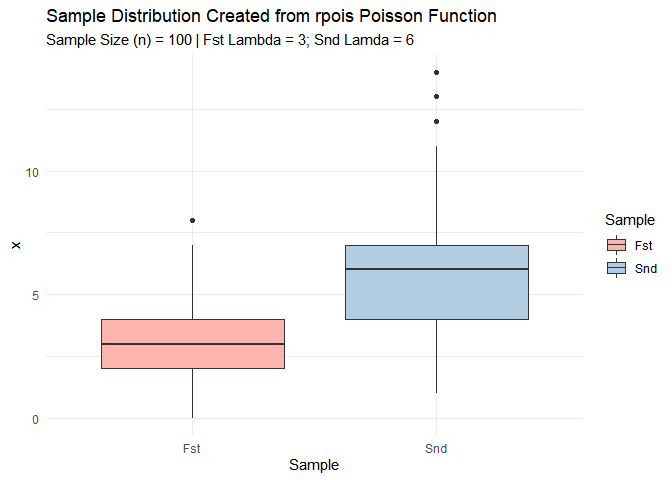
\includegraphics{lab2_files/figure-latex/boxplot-1.pdf}

\hypertarget{c-create-violin-plots}{%
\subsection{\texorpdfstring{\texttt{c} Create Violin
Plots}{c Create Violin Plots}}\label{c-create-violin-plots}}

\begin{Shaded}
\begin{Highlighting}[]
\NormalTok{basePlot }\SpecialCharTok{+} \FunctionTok{geom\_violin}\NormalTok{()}
\end{Highlighting}
\end{Shaded}

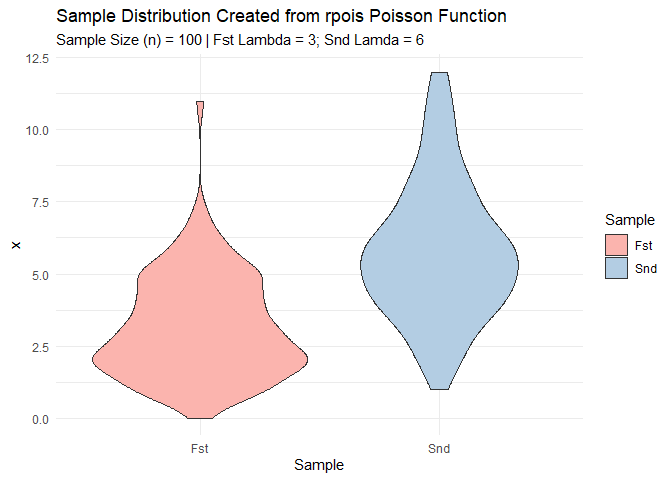
\includegraphics{lab2_files/figure-latex/violin-1.pdf}

\end{document}
